\documentclass[titlepage]{article}
\usepackage[pdftex]{graphicx}

% Title
\title{Lab 6: Electrons in Magnetic Fields/AC Circuits}
\author{Yacin Nadji}
\date{\today}

\begin{document}
\maketitle

\section{Statement of Objective}\label{sec:obj}
The objective of Lab \# 6, Electrons in Magnetic Fields/AC Circuits, was to observe its interaction with an external magnetic field, in order to determine the electron's charge to mass ratio. We also determined the relationships contained within a LRC circuit.

\section{Theory}\label{sec:theory}
\subsection{Part A: Charged Particles in Magnetic Fields}\label{sub:part_a_charged_particles_in_magnetic_fields-th}
A magnetic field, when penetrated by a charged particle, gives off a force onto said particle. This force is given by this Equation (\ref{eqn1})
\begin{equation}\label{eqn1}
	F = qv \times B
\end{equation}
Because of the nature of cross products ($\times$), the force will only be present if the velocity, ($v$), of the charged particle, and the magnetic field, ($F$), are \textbf{not} parallel. Conversely, when the particle and magnetic field are perpendicular, the particle will continue in circular motion, yielding Equation (\ref{eqn2})
\begin{equation}\label{eqn2}
	F = \frac{mv^2}{r}
\end{equation}
These two forces are equal to each other, setting them equivalent, yields Equation (\ref{eqn3})
\begin{equation}\label{eqn3}
	evB = \frac{mv^2}{r}
\end{equation}
The velocity of the electron is dependent upon the potential difference in the tube, due to the fact that the experiment took place inside a cathode-anode tube. Considering this, we can solve for the ratio of $\frac{e}{m}$, we algebraically determine Equation (\ref{eqn4})
\begin{equation}\label{eqn4}
	\frac{e}{m} = \frac{2V}{r^2 B^2}
\end{equation}
Where $V$ represents the potential difference in the tube.

The magnetic field in the experiment is provided by a Helmholtz coil, which is used with Equation (\ref{eqn5})
\begin{equation}\label{eqn5}
	B = \frac{8 \mu_0 IN}{5\sqrt{5}R}
\end{equation}
By substituting Equation (\ref{eqn5}) into Equation (\ref{eqn4}), we are presented with Equation (\ref{eqn6})
\begin{equation}\label{eqn6}
	\frac{e}{m} = \frac{125 V R^2}{32 \mu_0^2 I^2 N^2 r^2}
\end{equation}
If $I^2$ is plotted vs. $V$, it yields the slope
\begin{equation}\label{eqn7}
	slope = \frac{125 R^2}{32 \mu_0^2 N^2 r^2 \frac{e}{m}}
\end{equation}

\subsection{Part B: Alternative Current Circuit}\label{sub:part_b_alternative_current_circuit-th}
In an LRC circuit, the resonance condition of the circuit occurs when the current has reached its zenith. This only happens are specific angular frequencies, unique to that of the signal. These angular frequencies can be determined using Equation (\ref{eqn8})
\begin{equation}\label{eqn8}
	\omega = \frac{1}{\sqrt{LC}}
\end{equation}

\section{Equipment List}\label{sec:equipment_list}
\begin{itemize}
\item[*] Bainbridge Tube
\item[*] Helmholtz Coil
\item[*] DC Ammeter
\item[*] Power Supply
\item[*] Multimeter
\item[*] Resistor
\item[*] Capacitor
\item[*] Inductor
\item[*] Oscilloscope
\item[*] Sine Wave Function Generator
\end{itemize}

\section{Procedure}\label{sec:procedure}
\subsection{Part A: Charged Particles in Magnetic Fields}\label{sub:part_a_charged_particles_in_magnetic_fields-proc}
The radius of the Helmholtz coil was measured and recorded. The current through the Bainbridge tube was increased to an amperage between 3.5 and 4, but not exceeding 4A. The potential difference was then set to 30V. The current running through the Helmholtz coil was increased until the circular electron beam struck the furthest metal pin. This current was then recorded. The current was then increased and the current required for the electron beam to strike each metal pin was recorded. This process was then repeated for 50, 70, and 90V.

\subsection{Part B: Alternating Current Circuit}\label{sub:part_b_alternating_current_circuit-proc}
The capacitance of the capacitor was measured and recorded. The inductance of the inductor was also measured and recorded. The LRC circuit was then constructed. The leads from both channels of the oscilloscope were placed to measure the voltage across the resistor. The displace selector on the oscilloscope was changed to the x­y position and the Time/div knob was also placed in the x­y position. The leads were then changed so that channel 1 now measured the voltage across the whole circuit. The Lissajous figure was set up again and sketched. The frequency of the sine wave generator was turned up until the amplitude of the voltage across the resistor was at its maximum and the frequency recorded.

\section{Data}\label{sec:data}
\subsection{Part A: Charged Particles in Magnetic Fields}\label{sub:part_a_charged_particles_in_magnetic_fields-data}
First, let's get some generic measurements out of the way. The radius of the Helmholtz Coil was 31.75 cm $\pm$ 0.5 cm. The number of turns was $N = 100$. The following table shows the data collected dealing with the current required for the beam of electrons to strike each metal pin:

\begin{tabular}{ccccc}
\hline
 & 30 V & 50 V & 70 V & 90 V\\
\hline
$d_1 = 65mm$ & 1.98 A & 2.53 A & 3.03 A & 3.39 A\\
\hline
$d_2 = 78mm$ & 1.64 A & 2.13 A & 2.52 A & 2.85 A\\
\hline
$d_3 = 90mm$ & 1.41 A & 1.82 A & 2.15 A & 2.40 A\\
\hline
$d_4 = 103mm$ & 1.24 A & 1.62 A & 1.88 A & 2.13 A\\
\hline
$d_5 = 115mm$ & 1.11 A & 1.42 A & 1.67 A & 1.92 A\\
\hline
\end{tabular}

\subsection{Part B: Alternating Current Circuit}\label{sub:part_b_alternating_current_circuit-data}
The capacitor measured, 6.5nF, the inductor 0.96 H, and the resistor 51.1 k$\Omega$.

\subsubsection{Ch1 and Ch2 In Phase}\label{ssub:ch1_and_ch2_in_phase}
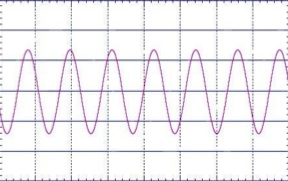
\includegraphics{1.jpg}

\subsubsection{Lissajous Graph Fig 1}\label{ssub:lissajous_graph}
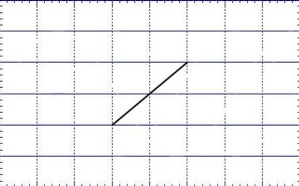
\includegraphics{2.jpg}

\subsubsection{Resistor Lagging 1/5ms}\label{ssub:resistor_lagging_1_5ms}
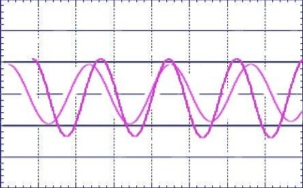
\includegraphics{3.jpg}

\subsubsection{Lissajous Graph Fig. 3}\label{ssub:lissajous_graph_fig_3}
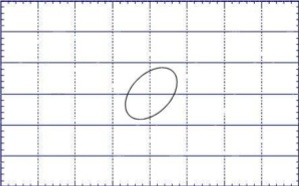
\includegraphics{4.jpg}

\section{Analysis of Data}\label{sec:analysis_of_data}
\subsection{Part A: Charged Particles in Magnetic Fields}\label{sub:part_a_charged_particles_in_magnetic_fields-aod}
\begin{center}\label{gph1}
	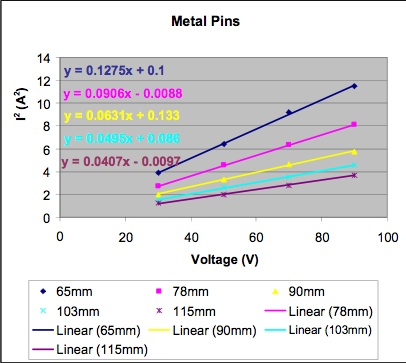
\includegraphics{5.jpg}
\end{center}

\begin{center}\label{tbl2a}
Metal Pins

\begin{tabular}{ccc}
\hline
Radius (m) & Slope & $\frac{e}{m}$\\
\hline
0.0325 & 0.1275 & 1.85 $\times 10^{11}$\\
\hline
0.0390 & 0.0906 & 1.81 $\times 10^{11}$\\
\hline
0.0450 & 0.0631 & 1.95 $\times 10^{11}$\\
\hline
0.0515 & 0.0495 & 1.89 $\times 10^{11}$\\
\hline
0.0575 & 0.0407 & 1.85 $\times 10^{11}$\\
\hline
\end{tabular}
\end{center}

The average experimental value for $\frac{e}{m}$ is $1.87 \times 10^{11}$ and the standard deviation is $4.84 \times 10^9$. The theoretical value is $1.76 \times 10^{11}$.

\subsection{Part B: Alternating Current Circuit}\label{sub:part_b_alternating_current_circuit-aod}
Since the frequency value we determined was the linear frequency, we must convert the collected data to be in angular frequency. We accomplished this using the following equation:
\[
	\omega = 2 \pi f
\]
The theoretical value was calculated using Equation (\ref{eqn8}).

\begin{center}\label{tblb1}
	Resonance Frequency $(Hz)$
	
	\begin{tabular}{cc}
	\hline
	Theoretical & 2014\\
	\hline
	Experimental & 2025\\
	\hline
	\end{tabular}
	
\end{center}

\section{Discussion of Results}\label{sec:discussion_of_results}
\subsection{Part A: Charged Particles in Magnetic Fields}\label{sub:part_a_charged_particles_in_magnetic_fields-dor}
With a theoretical value of $1.76 \times 10^{11}$, we can calculate the percent error:
\[
	\% Error = \frac{1.87 \times 10^{11} * 1.76 \times 10^{11}}{1.76 \times 10^{11}} * 100 = 6.4\%
\]
The margin of error is relatively small, considering the circumstances in which the amperage was measured. Had we conducted the experiment in a darker room, with some form of magnification to find the point the beam hits the metal pins, our \% error would've decreased significantly.

\subsection{Part B: Charged Particles in Magnetic Fields}\label{sub:part_b_charged_particles_in_magnetic_fields-dor}
Using the experimental and theoretical values, we can calculate the percent error:
\[
	\% Error = \frac{2025 - 2014}{2014} * 100 = 0.5\%
\]

\section{Conclusions}\label{sec:conclusions}
In conclusion, this lab successfully completed the objective outlined in \S \ref{sec:obj}. These results verified Equation (\ref{eqn4}) in proving the ratio, $\frac{e}{m}$, is equivalent to the relationship between $V, R, I, N, $ and $r$. The results also verified Equation (\ref{eqn8}) in that the angular frequency is inversely proportionate to the square root of LC.

\end{document}